\section{TADs \& leurs relations}
\subsection{Décomposition modulaire}

\bframes{
\small
4 modules (+ \texttt{main.c}) ont été créés pour la réalisation du TP\@:
\begin{enumerate}
    \item Le fichier \code{main.c} qui contient la fonction main qui va être la première instruction à exécuter. (Contient juste une boucle infinie \code{for (;;) \{ ... \}} qui va appeler les fonctions du module \code{shell} (notamment \code{sh\_getAndResolveCmd()}) pour interpréter l'entrée  utilisateur et exécuter les actions correspondantes. \\
    
    \item Le module \code{input} qui interprète l'entrée utilisateur, la parse, détermine si le job est à executer en foreground ou background... puis la passe au module \code{shell}\\
    

    \item Le module \code{shell}, le module principale de ce TP qui s'occupe de à peu près tout. Gestion de signaux, créations de processus avec \code{fork()}, gestion de ces processus, terminaisons \quo{clean} en attendant ses enfants et où en les forçant à se terminer\ldots \\

\end{enumerate}
}



\bframes{
\begin{enumerate}
    \stepcounter{enumi} \stepcounter{enumi} \stepcounter{enumi}

    \item Le module \code{files} (repris des TP03-5) \\
    S'occupe de la gestion fichers, (existence, type, taille etc.), des path des fichiers (absolute path, concatenation...) et de la gestion des erreurs liées à ces opérations.\\

    Ici seul \code{absPath()} et \code{concatPath()} ont été utilisées dans ce TP.
    
    \vspace{0.3cm}

    \item Le module \code{util} (repris des TP03-5) \\
      Fonctions / macros servant divers usages allant de la gestion d'erreurs à la gestion de chaînes de caractères, en passant par des wrappers qui incluent lesdites fonctions de gestions d'erreurs.\\
            
    \end{enumerate}
}

%

\subsection{Structures de données utilisées}
\bframes{
    Une structure de donnée (opaque) \code{Shell} a été implementé pour garder plus facilement trace (\textit{pid}) des tâches de fonds et de 1er plan en encapsulant le tout dans une structure.
    \bigskip

    La structure sert aussi à sauvegarder la dernière commande avec les\\ \code{argv} / \code{argc} correspondants afin de pouvoir la relancer si jamais cela est nécessaire. (e.g. en combinaison de l'utilisation du flag \code{SA\_RESTART} si une tâche de fond a été interrompu par un signal.)
}

\bframe{\footnotesize
\vspace{-0.2cm}

Voici à quoi la structure ressemble:\\
\vspace{0.15cm}
\code{shell.c}:
\vspace{-0.3cm}
\begin{figure}[!h]
    \centering
    %\hspace{-0.45cm}    
    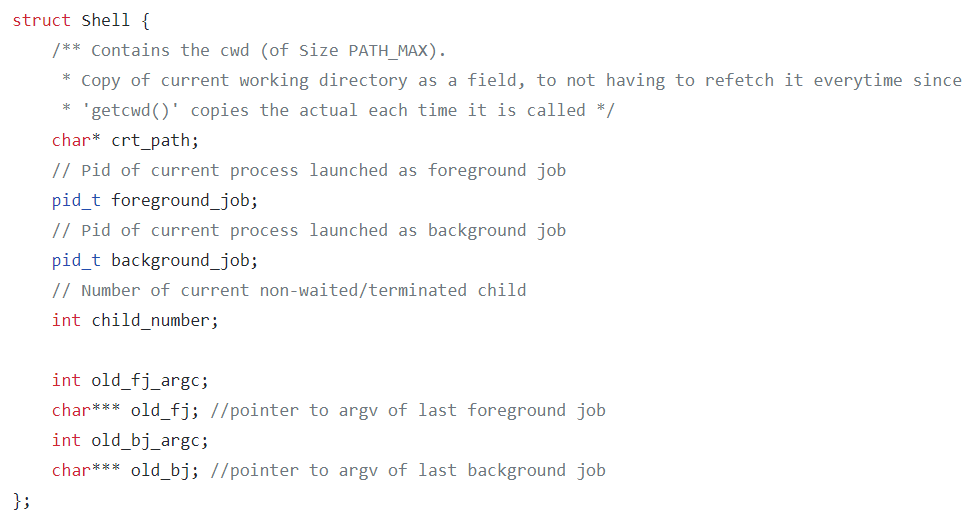
\includegraphics[width=12cm, height=6cm]{images/shell_struct.png}
    \caption{Module \code{shell}, structure \code{Shell} $\quad$(\code{shell.c}) \label{fig:shell1}}
\end{figure}
\unskip
}

%
%
\subsection{Décomposition fonctionnelle}
\bframes{
\small
    Une fois \quo{validée}, l'entrée utilisateur suit le \quo{chemin} suivant :
    \begin{enumerate}
        \item Comme dit précédemment, le module \code{input} se fait \quo{utiliser} par \code{shell} (fonction \code{sh\_getAndResolveCmd(Shell* sh)}) en parsant l'entrée etc avec la fonction \code{readParseIn(int* argc, int* isForeground)}
        
        \item dans \code{sh\_getAndResolveCmd}: on determine si la commande est built-in ou doit être executé en tant que job, puis appelle \code{cd()}, \code{exit\_shell()} ou \code{execute\_job(Shell*, char* cmd\_name, int isForeground})
        
        \item \code{execute\_job} va gérer les forks, update les attributs de la struct (tenir compte du nombre d'enfants de leurs pids...), refuser le \\ background job si on en a déjà un en cours, puis, si tout va bien, appelle la fonction \code{exec(Shell*, char* filename, char* argv[], int isForeground)} dans l'enfant créé.
        Si le job est à exécuter en foreground, le parent attend la mort de l'enfant avec \code{wait} (shell bloque).
    \end{enumerate}
}


\bframes{
    \begin{enumerate}
    \stepcounter{enumi} \stepcounter{enumi} \stepcounter{enumi}
        \item \code{exec} appelle \code{execvp(filename, argv)} avec les arguments qu'on lui a donné, puis \code{désattribue}les pids des foreground/background jobs de la struct shell (les mets à -2)

\vskip 7pt

        \item Quand un enfant meurt, il envoie un \code{SIGCHLD} à son processus parent, les signaux sont gérés avec les handlers définis avec \code{manage\_signals()} et \code{hdl\_sigint()}, \code{hdl\_sighup()}, \code{hdl\_sigchld()}.

        \code{hdl\_sigchld()} va \code{waitpid()} sur le child enregistré dans la struct qui a le pid correspondant puis va mettre ses attributs à jour.\\ Elle s'occupe aussi de relancer les appels interrompu par signaux.\\ (i.e. \code{errno == EINTR})
    \end{enumerate}
    }
    
\bframes{
\begin{enumerate}
 \stepcounter{enumi} \stepcounter{enumi} \stepcounter{enumi}
  \stepcounter{enumi} \stepcounter{enumi}
  
    \item Pour quitter proprement le shell à plusieurs fonctions. \code{clean\_exit(Shell*, int exitCode, int forceExit)} et \code{terminate\_all\_children(Shell*)}.
    
    \begin{itemize}
        \item \code{terminate\_all\_children()} est assez simple, elle va simplement \code{wait()} tant qu'il reste des enfants enregistré dans la struct.
        
        \item \code{clean\_exit()} quant à elle est un peu plus complexe, elle va, en fonction de \code{forceExit}, attendre le back/foreground job,
        \code{SIGTERM} le background job, \code{SIGTERM} le foreground job ou les 2.\\
        \vskip 5pt
        Ensuite, elle va appeler \code{terminate\_all\_children()}, puis \code{sh\_free(Shell*)} puis finalement \code{exit(exitCode)} avec le code qu'on lui a passé en argument.
        
    \end{itemize}
    
    
\end{enumerate}
}